\begin{recipe}
[ %
	preparationtime = {\SI{45}{\minute}},
%	bakingtime={\SI{1}{\hour}},
%	bakingtemperature={\protect\bakingtemperature{topbottomheat=\SI{280}{\celsius}}},
	portion = {\portion{4}},
	source = {Roosevelt}
    ]{Tom Yum Soup}

    \begin{figure}[p]
    	\centering
    	\makebox[\textwidth][c]{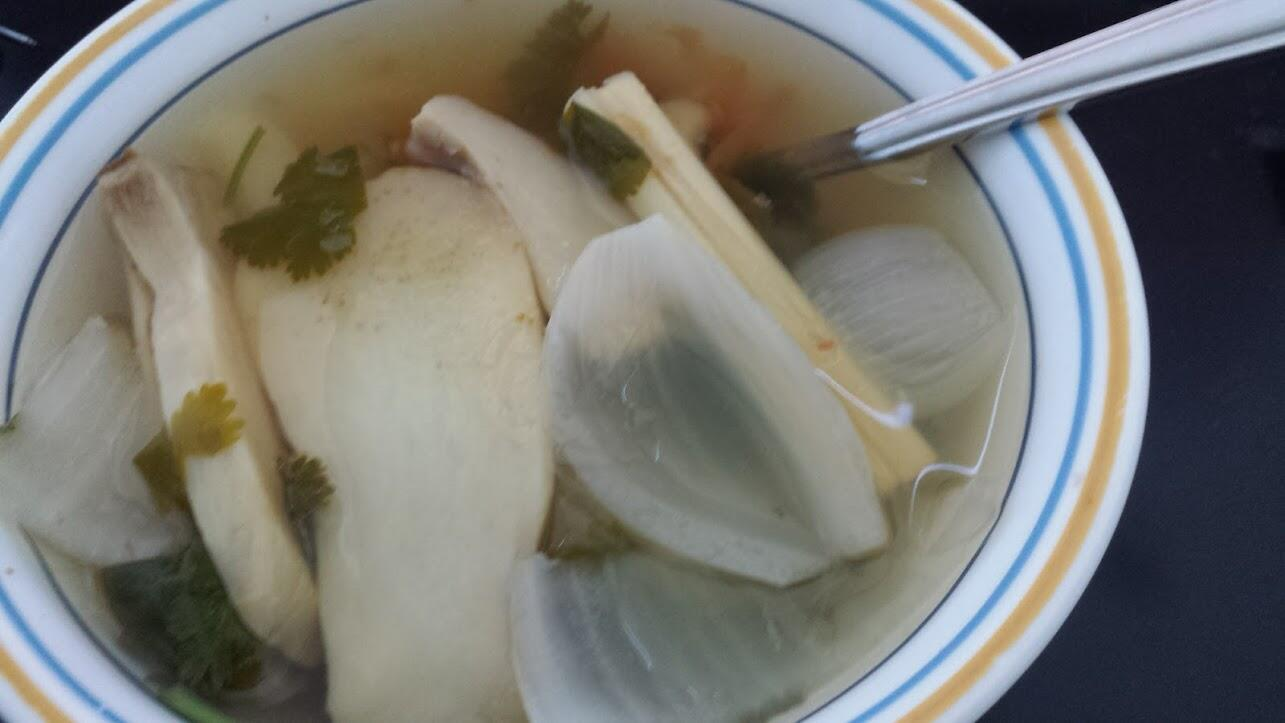
\includegraphics[height=\textheight]{tom_yum_soup/20170910_133512.jpg}}
    \end{figure}


    \introduction{
    	 I serve the soup over ramen style noodles, but I don't think that's standard.

    	 For mushrooms I use up to 2 pounds of whatever I can find including enoki, but this is up to you.
	}

	\ingredients[9]{
		\SI{8x1/2}{\cup} & Water \\
		\SI{4}{stalks} & Lemongrass \\
		\SI{1}{\inch} & Galangal \\
		\SI{10} & Lime leaves \\
		\SI{5}{cloves} & Garlic \\
		7 & Dried red chilies (adjust to your heat tolerance) \\
		& Lots of mushrooms \\
		2 & Tomatoes \\
		1 & Onion \\
		\SI{1}{\pound} & Shrimp \\
		\SI{8}{\tablespoon} & Fish sauce \\
		\SI{1}{\tablespoon} & Sugar \\
		2 & Limes (adjust depending on how sour you like it) \\
		& Cilantro
	}

	\preparation{

		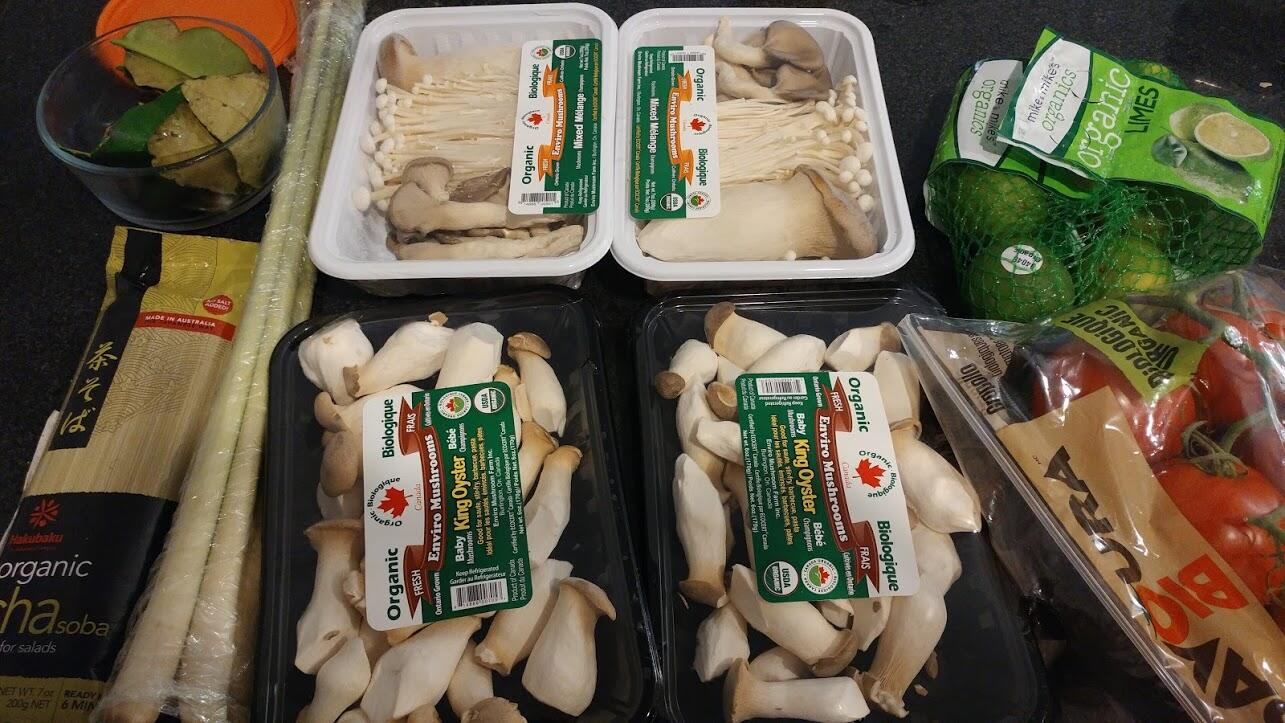
\includegraphics[width=0.52\textwidth]{tom_yum_soup/20191020_212427.jpg}

		\step Heat the water in a pot and add the lemongrass, galangal, lime leaves, garic and chilies. Simmer for \SI{10}{\minute}.

		\step Cut the tomatoes and onions into wedges. Add them to the pot along with the mushrooms and simmer for another \SI{2}{\minute}.

		\step Remove from heat and add the shrimp. The residual heat should cook or thaw whatever shrimp is being used, maybe with frozen raw shrimp you can run the heat a tiny bit.

		\step Add the fish sauce, sugar, limes and cilantro.
	}

\end{recipe}